%----------------------------------------------------------------------------------------
%	PACKAGES AND OTHER DOCUMENT CONFIGURATIONS
%----------------------------------------------------------------------------------------

\documentclass[11pt, oneside]{Thesis} % The default font size and one-sided printing (no margin offsets)

\graphicspath{{Pictures/}} % Specifies the directory where pictures are stored

\usepackage[square, numbers, comma, sort&compress]{natbib} % Use the natbib reference package - read up on this to edit the reference style; if you want text (e.g. Smith et al., 2012) for the in-text references (instead of numbers), remove 'numbers' 
\hypersetup{urlcolor=blue, colorlinks=false} % Colors hyperlinks in blue - change to black if annoying
\title{\ttitle} % Defines the thesis title - don't touch this

\begin{document}

\frontmatter % Use roman page numbering style (i, ii, iii, iv...) for the pre-content pages

\setstretch{1.3} % Line spacing of 1.3

% Define the page headers using the FancyHdr package and set up for one-sided printing
\fancyhead{} % Clears all page headers and footers
\rhead{\thepage} % Sets the right side header to show the page number
\lhead{} % Clears the left side page header
\pagestyle{fancy} % Finally, use the "fancy" page style to implement the FancyHdr headers

\newcommand{\HRule}{\rule{\linewidth}{0.5mm}} % New command to make the lines in the title page

% PDF meta-data
\hypersetup{pdftitle={\ttitle}}
\hypersetup{pdfsubject=\subjectname}
\hypersetup{pdfauthor=\authornames}
\hypersetup{pdfkeywords=\keywordnames}
\pagestyle{plain}


%----------------------------------------------------------------------------------------
%	TITLE PAGE
%----------------------------------------------------------------------------------------

\begin{titlepage}

\includegraphics[width=410pt]{ETSETB.jpg}
\begin{center}

\textsc{\LARGE \univname}\\[1.5cm] % University name
\textsc{\Large Master Thesis}\\[0.5cm] % Thesis type

\HRule \\[0.4cm] % Horizontal line
{\huge \bfseries \ttitle}\\[0.4cm] % Thesis title
\HRule \\[1.5cm] % Horizontal line
 
\begin{minipage}{0.4\textwidth}
\begin{flushleft} \large
\emph{Author:}\\
{\authornames} % Author name - remove the \href bracket to remove the link
\end{flushleft}
\end{minipage}
\begin{minipage}{0.4\textwidth}
\begin{flushright} \large
\emph{Supervisor:} \\
{\supname} % Supervisor name - remove the \href bracket to remove the link  
\end{flushright}
\end{minipage}\\[6cm]

%\large \textit{A thesis submitted in fulfilment of the requirements\\ for the \degreename}\\[0.3cm] % University requirement text
%\textit{in the}\\[0.4cm]
\groupname\\\deptname\\[2cm] % Research group name and department name
 
{\large \today}\\[4cm] % Date
%\includegraphics{Logo} % University/department logo - uncomment to place it
 
\vfill
\end{center}

\end{titlepage}


%----------------------------------------------------------------------------------------
%	ABSTRACT PAGE
%----------------------------------------------------------------------------------------

\addtotoc{Abstract} % Add the "Abstract" page entry to the Contents

\abstract{\addtocontents{toc}{\vspace{1em}} % Add a gap in the Contents, for aesthetics

During the last years, Visible Light Communication (VLC), a novel technology that enables standard Light-Emitting-Diodes (LEDs) to transmit data, is gaining significant attention. In the near future, this technology could enable devices containing
LEDs – such as car lights, city lights, screens and home appliances – to carry information or data to the end-users, using their smartphone. However, VLC is currently limited by the end-point receiver, such as a the mobile camera, or a peripheral connected through the jack input and to unleash the full potential of VLC, more advanced receiver are required.

On other, few year ago, Google ATAP - the Google innovation department - announced the Ara initiative. This consist on a modular phone where parts of the phone, like cameras, sensors or networks can be changed. So when a new feature appears or required by the user it is not needed to change the mobile phone, just to buy the modules with the functionality.

This Master Thesis presents the design and development of a simple module that will support communication by light (VLC) using the Ara Module Developer Kit provided by Google. It consists on building a front-end circuit, connecting a photodiode that receives the level of light and use it as data carrier, in order to receive and display data inside a custom Android application on the Ara smartphone.

}

\clearpage % Start a new page

%----------------------------------------------------------------------------------------
%	ACKNOWLEDGEMENTS
%----------------------------------------------------------------------------------------

\setstretch{1.3} % Reset the line-spacing to 1.3 for body text (if it has changed)

\acknowledgements{\addtocontents{toc}{\vspace{1em}} % Add a gap in the Contents, for aesthetics

To my supervisor, Josep Paradells who trust me and give me the opportunity to work on this project.
\newline To the Wireless Network Group team for there guidance and everyday help and support.
\newline To Miguel and Cleo, my hosts during these five past months in Barcelona.
\newline And finally, to Rtone company and Adrien Desportes, its Chief Executive Officer, who offer me a joint-PhD position with the CITI lab, to dig deeper into the Visible Light Communication subject.
}

\clearpage % Start a new page

%----------------------------------------------------------------------------------------
%	LIST OF CONTENTS/FIGURES/TABLES PAGES
%----------------------------------------------------------------------------------------

\pagestyle{fancy} % The page style headers have been "empty" all this time, now use the "fancy" headers as defined before to bring them back

\lhead{\emph{Contents}} % Set the left side page header to "Contents"
\tableofcontents % Write out the Table of Contents

\lhead{\emph{List of Figures}} % Set the left side page header to "List of Figures"
\listoffigures % Write out the List of Figures

\lhead{\emph{List of Tables}} % Set the left side page header to "List of Tables"
\listoftables % Write out the List of Tables

%----------------------------------------------------------------------------------------
%	ABBREVIATIONS
%----------------------------------------------------------------------------------------

\clearpage % Start a new page

\setstretch{1.5} % Set the line spacing to 1.5, this makes the following tables easier to read

\lhead{\emph{Abbreviations}} % Set the left side page header to "Abbreviations"
\listofsymbols{ll} % Include a list of Abbreviations (a table of two columns)
{
\textbf{ADC} & \textbf{A}nalogic to \textbf{D}igital \textbf{C}onverter \\
\textbf{BPS} & \textbf{B}it \textbf{P}er \textbf{S}econd \\
\textbf{DMA} & \textbf{D}irect \textbf{M}emory \textbf{A}ccess \\
\textbf{I\textsuperscript{2}C} & \textbf{I}nter\textbf{I}ntegrated \textbf{C}ircuit \\
\textbf{MDK} & \textbf{M}odule \textbf{D}evelopement \textbf{K}it \\
\textbf{MCU} & \textbf{M}icro \textbf{C}ontroller \textbf{U}nit \\
\textbf{Op-Amp} & \textbf{O}perational \textbf{A}mplifier \\
\textbf{OS} & \textbf{O}perating \textbf{S}ystem \\
\textbf{OOK} & \textbf{O}n \textbf{O}ff \textbf{K}eying \\
\textbf{PTM} & \textbf{P}ulse \textbf{T}ime \textbf{M}odulation \\
\textbf{PAM} & \textbf{P}ulse \textbf{A}mplitude \textbf{M}odulation \\
\textbf{PWM} & \textbf{P}ulse \textbf{W}idth \textbf{M}odulation \\
\textbf{RAM} & \textbf{R}andom \textbf{A}ccess \textbf{M}emory \\
\textbf{SDK} & \textbf{S}oftware \textbf{D}evelopement \textbf{K}it \\
\textbf{TIA} & \textbf{T}rans \textbf{I}mpedance  \textbf{A}mplifier \\
\textbf{UART} & \textbf{U}niversal \textbf{A}synchronous \textbf{R}eceiver \textbf{T}ransmitter\\
\textbf{VLC} & \textbf{V}isible \textbf{L}ight \textbf{C}ommunication \\
}

%----------------------------------------------------------------------------------------
%	THESIS CONTENT - CHAPTERS
%----------------------------------------------------------------------------------------

\mainmatter % Begin numeric (1,2,3...) page numbering

\pagestyle{fancy} % Return the page headers back to the "fancy" style

% Include the chapters of the thesis as separate files from the Chapters folder
% Uncomment the lines as you write the chapters

% Introduction

\chapter{Introduction} % Main chapter title

\label{Chapter1} % For referencing the chapter elsewhere, use \ref{Chapter1} 

\lhead{Chapter 1. \emph{Introduction}} % This is for the header on each page - perhaps a shortened title
	
%----------------------------------------------------------------------------------------
%	MOTIVATION
%----------------------------------------------------------------------------------------

\section{Motivations}

For the last century, radio frequency (RF) has dominated wireless communications.But RF has been a victim of its own success. The number of mobile devices and embedded systems has increased tremendously as technology becomes a primary need in peoples lives. This explosion of mobile devices comes at a cost:the frequency spectrum is a scarce resource. The massive increase in RF communicating devices is leading to a saturation of the available bandwidth, which will  result in a drop of quality-of-service.

To ameliorate the bandwidth saturation problem, the research community has been exploring other wireless technologies. One of the most promising alternatives is visible light communication. Light is electromagnetic radiation just like RF, but the difference lies in frequency. Because of this frequency, the interaction between light and matter is different on a fundamental level which gives light unique properties.

With the advent of Visible Light Communication (VLC), the widespread exploitation of the visible light spectrum is becoming a reality. VLC enables standard
Light Emitting Diodes (LEDs) to transmit data wirelessly, and this is an important step because LEDs are permeating our daily environments at a very fast pace.

After intensive research into energy consumption, in 2009 the European Union and other countries started measures to phase out incandescent light bulbs in
favor of high efficient LEDs. But it is not only residential and commercial lighting that is being replaced with LEDs, a number of other objects such as car lights,
city lights, billboards, smartphone and laptop screens, price tags, toys and home appliances, are also using LEDs to reduce their energy consumption.

A nice VLC example is indoor positioning. At the 2014 Mobile Wolrd Congress (MWC 14'), the i2CAT foundation demonstrate its indoor location positioning system, using VLC and the phone's ambient light sensor.

Other applications, such navigation assistance for visually impaired, propose an other approach using an external peripheral as VLC receiver, plug-in it to the jack mobile phone or through Bluetooth \citep{bluereceiver}.

Thus, considering that VLC can potentially transform any LED device into a wireless transmitter there may be a new generation of objects waiting to be connected to people smartphone.


%----------------------------------------------------------------------------------------
%	OBJECTIVES
%----------------------------------------------------------------------------------------

\section{Objectives}
However, actual research and VLC implementation on mobile phone are highly limited by receiver hardware. In fact, embedded sensor on smartphone, such as camera are not appropriate for sensing modulated light. External peripheral, adding an other channel reduce considerably the throughput.
That why, the recent concept of modular smartphone, called Phonebloks (2013) and industrialized as Project Ara y Google, could be the solution.

Project Ara is an effort in Google's Advanced Technology Projects (ATAP) organization to create a modular smartphone platform, with the twin aims of delivering a deep customization experience to users and enabling significantly lowered barrier to entry into the mobile hardware ecosystem.

This project aims to take advantage of this new technology developing a Visible Light Communication receiver for the Ara plartform. Major objectives are listed below :
\begin{itemize}
\item Design and develop a module that support visible light communication.
\item Determine the Ara smartphone possibility for future work on wireless communications.
\item Develop a convenient LED driver suited for our need. 
\item Experiment a communication between a LED emitter and the modular smartphone.
\end{itemize}


%----------------------------------------------------------------------------------------
%	ORGANISATION
%----------------------------------------------------------------------------------------

\section{Report Organization}

Chapter 1 of this report serves to provide an introduction of the basic concepts and techniques and also shows several designs that are required for the implementation of VLC.  \\
Chapter 2 provides the background needed for the VLC designs. \\ 
Chapter 3 provides the literature review of the VLC technology. \\ 
Chapters 4 and 5 provide our proposal description and the experimental setup and implementation of the models. \\
Chapter 6 presents our results and recommendations for improving the designs as well as the conclusion with suggestions for further improvements in the work.
% Technical background}
\chapter{Technical background}
\label{Technical}

\lhead{Chapter 2. \emph{Technical background}}

\section{VLC Standard}
VLC as we know it today would not be possible without LEDs. Before we introduce
our proposal, we provide background information
about LEDs as wireless transmitter, then we describe the many ways in which
light intensity can be modulated and received, and the line coding scheme used
in indoor VLC.

\section{VLC Technology}

Modulation of light has been used for centuries. In 1792 the French inventor
Claude Chappe invented the optical telegraph, a system of towers with signaling
devices, which allowed Napoleon to pass messages throughout his empire. Although
simple and practical, these systems are the ancestors of VLC. For some decades
after these events, light communication in the form of morse was used, but further
development of light communication stood still because with incandescent lamps
the data rates pale in comparison to what could be achieved with radio.

It is only until recently that we have a pervasive infrastructure that can modulate
light to achieve data rates that are meaningful for today’s communication needs.
Due to recent advancements in LED technology we can transform light bulbs into
high speed wireless transmitters. Data can be modulated in every light source
using changes in intensity, but only certain light sources possess the necessary
properties to transmit high data rates.

Fundamentally, modulating light requires changes of light intensity. For the last
century incandescent lamps have been the primary source of light, but incandescent
light cannot comply with high speed modulation because of the mechanism
it uses to generate light. Incandescence is the effect of emitting thermal radiation
from matter as a result of its temperature. In incandescent light bulbs a wire is
heated by running a current through it, and the resistance of this wire forms kinetic 
energy which is released in the form of light. This means that intensity control
of incandescent lamps takes place through two steps, resulting in indirect control
of the signal. This would not be a problem if the thermal inertia would not make
the system too slow for high speed modulation, but it does.

In the case of LEDs, the direct relation between intensity and electricity permit
high speed modulation. LEDs consist of a semiconductor material that contains
excited electrons. A fundamental property of electrons is that when they are
forced into a lower energy state they release their energy in the form of the emission
of photons. This effect is called electroluminescense and gives direct control
over light intensity through the control of voltage and current. A simple circuit
with transistors can deliver the necessary control of current, and this makes the
changes in light intensity fast enough to transfer information at a high data rate.

An alternative to LEDs is laser. Lasers can also be controlled at high speed, and
have the additional capability of strengthening the electroluminescense effect by
amplifying and focusing the generated light. This makes laser a good candidate
for long range communication, but for short distances its transmission angle is too
narrow (and hence it can be easily obstructed) without using lenses. Another
important disadvantage of laser is that poses health hazards to human beings.

\subsection{Modulation and transmitter}

The light emitted by LEDs can be modulated in different forms, and there are also
several types of receivers that can be used to decode the modulated light. Next,
we describe all these options.

As mentioned before, the ability of LEDs to modulate light at high speeds make
them the obvious choice for VLC transmitters in terms of speed and light intensity,
but potentially good transmitters are not the only thing that make a communication
system work. Data needs to be encoded (or modulated) into a signal before
transmission.
In radio communication, two common parameters used in signal modulation
are amplitude and frequency. Although radio and light are both electromagnetic
waves, the effect of modulation is not the same. We will briefly describe this point
to make the reader aware of the fundamental difference in modulation between
radio and VLC.

In radio, frequency modulation changes the frequency of the waves in the electromagnetic
field, and amplitude modulation changes the height of this waves.
In VLC, amplitude modulation works the same way as in radio, and it is often
called intensity modulation. Frequency modulation however, is very hard to apply
with visible light. It can be done but requires advanced laser setups to change
the signal’s properties, like phase and frequency, through interference. Instead,
when people talk about frequency modulation in VLC, they mean that the intensity
is shaped into a high frequency signal. By varying the frequency of this intensity
pulses, we get frequency modulation.

So, frequency modulation in VLC is actually frequency modulation through amplitude
modulation. This is the main difference between radio and light modulation.

There are many different modulation schemes in use for VLC, and we will now
discuss the most commonly used.

\begin{enumerate}

\item On-Off-Keying (OOK), or amplitude shift keying, uses keying (switching) to
turn a carrier signal on and off. OOK has a low processing burden but is
proven to be very sensitive to noise. Enhanced schemes like On-Off-Keying
Non-Return-to-Zero have shown data rates of 1.5 Gigabits per seconds,
using a Integrated Circuit with LEDs bonded into the chip \citep{ook-450}.

\item Pulse Time Modulation (PTM) is a technique in which data is modulated
in the ratio between the on and off time of the carrier signal. Pulse Position
Modulation (PPM) and Pulse Width Modulation (PWM) fall into this
category. The advantage of PTM is that it does not require digital-to-analog
converters to generate a smooth output signal, and does not require an
analog-to-digital converter either but only a comparator circuit. On the other
hand, PTM requires accurate timing for both the receiver and transmitter
because the ratio between on and off periods needs to be well synchronized.
Another advantage of PTM is that it provides flickering and dimming
support without additional techniques, which is good for use in illumination
devices, but speeds are lower than with other modulation systems \citep{ppm}.


\item  Pulse Amplitude Modulation (PAM) uses brightness levels to realize multilevel
signals to encode symbols. This modulation is sensitive to external
light sources as they influence the intensity, and has relative low speeds
compared to other techniques. Dimming control can easily be implemented
in PAM by changing the probability of the constellation points \citep{diming}
iv Frequency Shift Keying (FSK) looks a lot like On-Off-Keying, but instead of
switching a carrier on and off, the system switches between two frequencies.
This switch in frequency can be in terms of color i.e. a one is red and
a zero is blue, or in pulse frequency.

\item Phase Shift Keying (PSK) encodes symbols by changing the phase of the
light intensity that has been shaped into a sinusoidal form. Many variants
of PSK exist, depending on the number of constellation points used (Binary
PSK uses 2 points, 0\degree  and 180\degree , Quadrature PSK uses 4 points). PSK
can be used as base modulation, but can also be used in combination
with other techniques like OFDM to improve certain weaknesses like intersymbol
interference \citep{ofdm-plc}.

\item Orthogonal Frequency Division Multiplexing (OFDM) is a technique that
uses a large number of modulated carriers with sufficient frequency spacing
so that they are orthogonal. Again, this frequency is modulated through intensity.
The strongest advantage of OFDM is that it provides resistance to
multipath effects, which result in long distances and high speed data transfers.
Data rates beyond 3 Gigabit per seconds have been reported at short
distances $\approx$ 10cm) \citep{modulationStandard}. Unfortunately such high speeds demand require
high-speed processing units.

\item  Quadrature Amplitude Modulation (QAM) is a modulation scheme that conveys
bit streams by changing the amplitudes of two or more independent
carrier signals, which results in a spectral efficient scheme. A form of
QAM is the Carrier-less Amplitude and Phase (CAP) modulation, a promising
high speed VLC modulation scheme capable of transmitting at 3.22
gigabits per second using an RGB-type led. QAM and CAP can both
be combined with OFDM to improve its performance even further \citep{ofdm-cap}.

To select a good modulation scheme, people have designed models that can
be used to compare different schemes by simulating environmental conditions.
The Matlab-based platform of De Lausnay et al. evaluates different modulation
techniques and can also help to select the right modulation type \citep{matlab}.

Based on the information above, we decided to use On-Off-Keying modulation
for our platform because of the good average performance. The use of this technique keeps component count low so that multiple transmitters and receivers fit on the board.

\end{enumerate}

\subsection{Receivers}

While on the transmitter side the most widely used element is the LED, on the
receiver side we have several options: cameras, photodiodes and phototransistors,
and LEDs themselves. The common name for these types of sensors is
photodetectors and they use the same fundamental principle, the photoelectric
effect: many metals release electrons when light shines upon it. Although these
sensors share the same effect, they have subtle differences that result in unique
characteristics.

\begin{enumerate}

\item Cameras can detect light, its intensity and its color, using an array of semiconductor
junctions or capacitors. As the miniaturization of cameras continues
they can be found in embedded systems like mobile phones, allowing
them to receive vlc signals without additional hardware \cite{camera}. Cameras have
the advantage of focusing on the transmission source by looking at specific
pixels, so it becomes possible to select a specific VLC source or to ignore
a noise source. As a receiver for VLC, cameras have the disadvantage
of requiring more processing to retrieve the signal from the image sensor.
Secondly, a bigger disadvantage is the frame rate which is limited by the
camera’s (electronic or mechanic) shutter speed, which limits the signal
sample rate and thus the data transfer rate. There are high speed
cameras which offer a solution to this problem, but currently they are
too big and power hungry to use in embedded devices.

\item Photodiodes and phototransistors work based on the same principle but
their assembly is different: photodiodes have only one metal junction and
transistors have two. This semiconductor junction is exposed through a
transparent casing, so photons can reach the junction and, when having
the right frequency, excite electron-hole pairs which results in a current and
voltage. Because of the big surface of the semiconductor junction, photodiodes
and phototransistors are very sensitive to light. When comparing
photodiodes to phototransistors, diodes are faster due to the single junction
giving it a fast response time. On the other hand, phototransistors have a
bigger signal gain which results in a stronger electric signal. A disadvantage
of photodiodes is the dedicated circuitry needed for amplification, filtering
and sampling to be able to receive a clear electronic signal. Advances in
technology are capable of integrating these into a single chip which can
alleviate this disadvantage.

\item LEDs can be used as light sensors. An attentive reader may have noticed that photodiodes and LEDs exploit an oppose effect: while in photodiodes photons that strike the material generate a flow of electrons, in LEDs a flow of electrons release photons (light). This reversed and complementary effect can be used to make an LED both a receiver and a transmitter of VLC \citep{led2led}.

Considering the various options for receivers, we opted for photodiodes because
they have the higher potential to achieve high data rates, are more sensitive
than other sensors.

\end{enumerate}

\subsection{Line coding}

IEEE 802.15.7 standard suggests use different lines for VLC PHY I, that can be use with OOK or VVMN modulation.

\subsubsection{Manchester}

\subsubsection{4B6B}

\subsubsection{8B10B}


\section{Ara Plateform}
\subsection{Introduction to the Ara project}

Project Ara is the codename for an initiative that aims to develop an open hardware platform for creating highly modular smartphones. The platform will include a structural frame or endoskeleton that holds smartphone modules of the owner's choice, such as a display, camera or an extra battery. It would allow users to swap out malfunctioning modules or upgrade individual modules as innovations emerge, providing longer lifetime cycles for the handset, and potentially reducing electronic waste. Project Ara smartphone will begin pilot testing in Puerto Rico later 2015 with a target bill of materials cost of \$ 50 for a basic grey phone. The project was originally headed by the Advanced Technologies and Projects team within Motorola Mobility while it was a subsidiary of Google. Although Google had sold Motorola to Lenovo, it is retaining the project team who will work under the direction of the Android division.

\subsection{Project goals}
Google says the device is designed to be utilized by "6 billion people"; including 1 billion current smartphone users, 5 billion feature phone users, and 1 billion future user not currently connected. Google intends to sell a starter kit where the bill of materials is \$ 50 and includes a frame, display, battery, low-end CPU and WiFi.

Google wants Project Ara to lower the entry barrier for phone hardware manufacturers so there could be "hundreds of thousands of developers" instead of the current handful of big manufacturers. This would be similar to how the Google Play Store is structured. Lowering the barrier for entry allows many more people to develop modules. Anyone will be able to build a module without requiring a license or paying a fee.

\subsection{Structure and features}

Ara Smartphones are built using modules inserted into metal endoskeletal frames known as "endos". The frame will be the only component in an Ara Smartphone made by Google.It acts as the switch to the on-device network linking all the modules together. Two frame sizes will be available at first: "mini", a frame about the size of a Nokia 3310 and "medium", about the size of a LG Nexus 5.In the future, a "large" frame about the size of a Samsung Galaxy Note 3 will be available. Frames have slots on the front for the display and other modules. On the back are additional slots for modules. The data from the modules can be transferred at up to 10 gbps connection. The 2x2 modules have two connections and will allow up to 20 gbps. However, this stack isn't yet included in the Ara Development Kit, that only uses standard I/O such as UART or I$^2$C, providing lower transfer rate.

Modules can provide common smartphone features, such as cameras and speakers, but can also provide more specialized features, such as medical devices, receipt printers, laser pointers, pico projectors, night vision sensors, or game controller buttons. Each slot on the frame will accept any module of the correct size. The front slots are of various heights and take up the whole width of the frame. The rear slots come in standard sizes of 1x1, 1x2 and 2x2. Modules can be hot-swapped without turning the phone off. The frame also includes a small backup battery so the main battery can be hot-swapped.Modules are secured with electropermanent magnets. The enclosures of the modules were planned to be 3D-printed, but due to the lack of development in the technology Google opted instead for a customizable molded case.

Modules will be available both at an official Google store and at third-party stores. Ara Smartphones will only accept official modules by default, but users can change a software setting to enable unofficial modules. This is similar to how Android handles app installations.

\subsection{Project team}

Project Ara was developed and is led by Paul Eremenko from Google ATAP. The core Project Ara team at Google consists of three people with most of the work being done by outside contractors. One of the main contractors is NK Labs, a Massachusetts-based engineering firm, whose co-founder is Ara Knaian after whom the project was named. Another contractor is 3D System.

\subsection{History and development process}

The first version of the developers' kit relies on a prototype implementation of the Ara on-device network using the MIPI UniPro protocol implemented on FPGA and running over an LVDS physical layer with modules connecting via retractable pins. Subsequent versions will soon be built around a much more efficient and higher performance ASIC implementation of UniPro, running over a capacitive M-PHY physical layer.
         
\subsection{Architecture}

\subsubsection{Android AP board}

The Application Processor Board is development kit for the Android Operating system giving convenient way to modify or update the OS.

The plateform is base

\begin{figure}[htbp]
  \centering
    \scalebox{0.4}{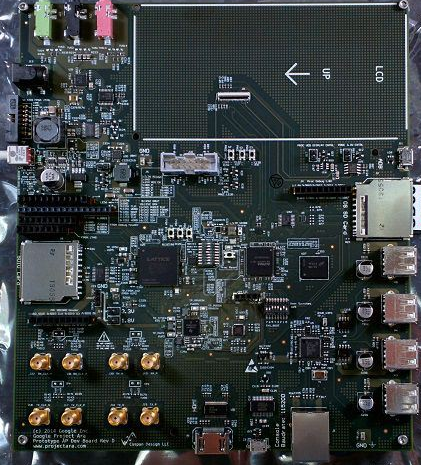
\includegraphics[width=\textwidth]{Pictures/APDevBoard.png}}
    \rule{35em}{0.5pt}
  \caption[Ara Application Processor Board]{Ara Application Processor Board}
  \label{fig:ap-board}
\end{figure}

\subsubsection{Endoskeleton}

\begin{figure}[htbp]
  \centering
    \scalebox{0.4}{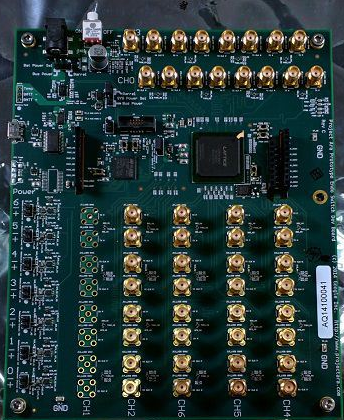
\includegraphics[width=\textwidth]{Pictures/endo.png}}
    \rule{35em}{0.5pt}
  \caption[Ara Endoskeleton Switch Board]{Ara Endoskeleton Switch Board}
  \label{fig:endo}
\end{figure}

\subsubsection{GP Endpoint board}

\begin{figure}[htbp]
  \centering
    \scalebox{0.4}{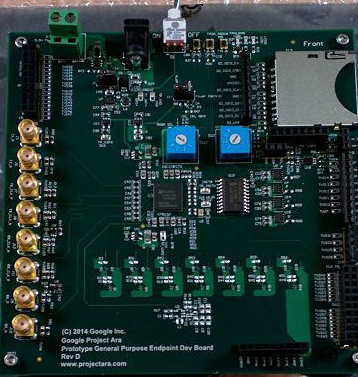
\includegraphics[width=\textwidth]{Pictures/genericendpoint.png}}
    \rule{35em}{0.5pt}
  \caption[Ara Generic Endpoint Board]{Ara Generic Endpoint Board}
  \label{fig:gpendpoint}
\end{figure}

 
% State of the Art

\chapter{State of the Art} % Main chapter title

\label{SoA} % For referencing the chapter elsewhere, use \ref{Chapter1} 

\lhead{Chapter 3. \emph{State of the Art}} % This is for the header on each page - perhaps a shortened title

This chapter provides an overview of the topics that supplied the ideas for this thesis. The
following sections examine the previous works which have been done on implementing
Visible Light Communication technology.

%----------------------------------------------------------------------------------------
%	VLC
%----------------------------------------------------------------------------------------

\section{VLC Implementations}

\subsection{Visible Light Communication System Considered}

An indoor visible light communication system using white LEDs under consideration is
shown in Fig. 3.1 and 3.2 [1]. All the lights in the room are replaced by LEDs. The LEDs
are not only used for illuminating the room but also for an optical wireless
communication system. On-off Keying Return-to-Zero (OOK-RZ) coding is used for
modulating white LEDs. Optical lighting and optical transmission of the white LEDs
have been tested to evaluate the requirements of using VLC for indoor applications. The
effects of the delay problems faced in the high data rate transmission have been studied
and presented [1].

Fig 3.1: VLC model room [1]. Fig 3.2: Distribution of LEDs inside model room [1].

\subsection{Visible Light Road-to-vehicle Communication Using High-Speed Camera}

LEDs are already being used in traffic lights, and they can be used as the communication
medium. Road-to vehicle communication using the LEDs in the traffic signal lights was
proposed.

Figure 3.3: Road-to-vehicle visible light communication [17].

The above Fig. 3.3 shows the basic usage of LED as a transmitter and CAMERA as a
receiver. In this model, they mounted a camera before the front end of the car. The
camera is used as the information receiver from traffic signal lights. The advantage of
using the camera is that multiple data can be transmitted by the LEDs and received by
High-speed cameras [17]. 


\subsection{Integrated System of White LED Visible-Light Communication and Power-Line Communication}

In [2], optical communication using the existing power-line in a household is proposed as
shown in \ref{fig:vlc-model}

\begin{figure}[htbp]
  \centering
    \scalebox{0.6}{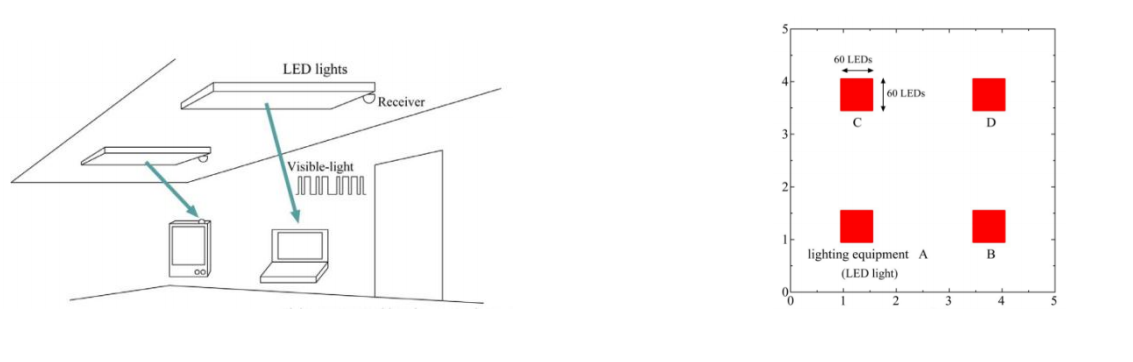
\includegraphics[width=\textwidth]{Pictures/vlc-model-room.png}}
    \rule{35em}{0.5pt}
  \caption[VLC System model]{VLC System model}
  \label{fig:vlc-model}
\end{figure}

The power-line is used for communication between white LEDs and other fixed
networks. The already installed power-lines and outlets behave as data networks and
ports.

\begin{figure}[htbp]
  \centering
    \scalebox{0.6}{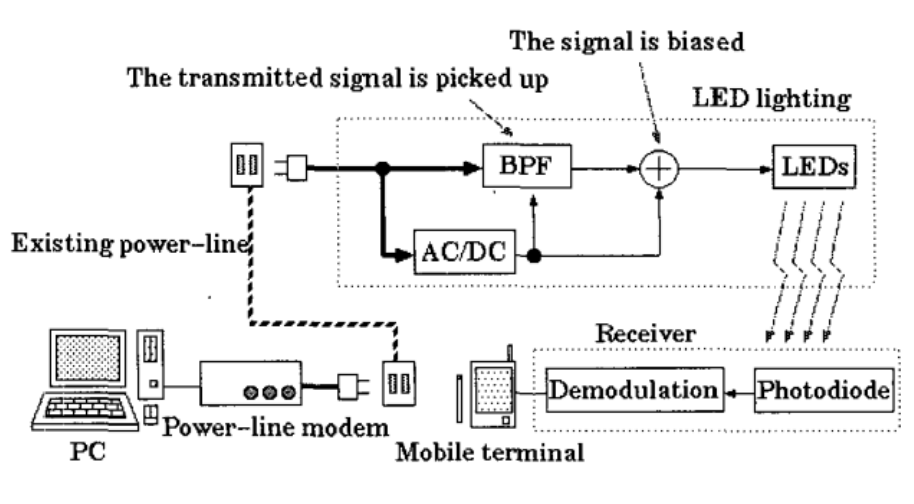
\includegraphics[width=\textwidth]{Pictures/vlc-powerline.png}}
    \rule{35em}{0.5pt}
  \caption[Waveform on power-linel]{Waveform on power-line}
  \label{fig:vlc-powerline}
\end{figure}

As in optical intensity modulation, the transmitted signals are added to the cyclic
waveform of the alternating current (AC). The transmitter signal from the PC is picked
by BPF through the power-line, and biased before sending to the LED lights. The
electrical signal is then converted into an optical signal by LEDs and sends it to the
photodiode, where it converts the captured optical signal to an electrical signal. The
signal is demodulated according to the received level of light and then is passed to the
mobile terminal [2].

\subsection{Visible Light Communication for Advanced Driver Assistant Systems}

\begin{figure}[htbp]
  \centering
    \scalebox{0.6}{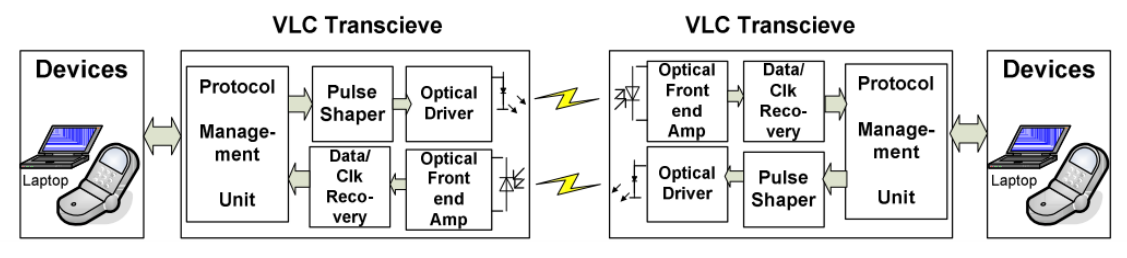
\includegraphics[width=\textwidth]{Pictures/vlc-driver.png}}
    \rule{35em}{0.5pt}
  \caption[General architecture for a full duplex VLC system ]{General architecture for a full duplex VLC system }
  \label{fig:vlc-driver}
\end{figure}

Optical communications for outdoor communication has been discussed and elaborated
upon [4]. Devices such as laptops and mobile phones can be used for transmitting and
receiving information, using transceivers, as shown in \ref{fig:vlc-driver}. Transceiver systems use
both LEDs and photodiodes. Intensity modulation was implemented to reach the most
viable modulation. Various important design parameters were optimized by using
intensive investigation based on gain variation over 100m of transmission range [4]. 


\subsection{Dual-Use Visible Light Approach to Integrated}

Communication and Localization of Underwater Robots with
Application to NonDestructive Nuclear Reactor Inspection
A VLC system for wireless underwater communication was proposed in [23] for robotic
inspection of nuclear power plants; there the reactor exists in an underground
environment as shown in Fig. 3.7. A solution for maintaining the consistent line of sight
to maintain a communication link was discussed in detail in [23].

Figure 3.7: Architecture of the dual-use optical communication system [23].

An optical wireless link has been established between the Remotely Operated Vehicles
(ROV) and gateway station using LEDs and Photodiodes on both sides as depicted in Fig
3.7. Underwater ROV was used to communicate with the gateway station over water to
transmit control signals. Both the gateway station and ROV are capable of directing a
light beam in the three-dimensional space [23]. 


\subsection{Study of Visible Light Communication System Using RGB LED Lights}

Figure 3.8: Outline of the system [24].

A prototype was designed to demonstrate wireless VLC using RGB LEDs and sensors
[24]. As shown in Fig. 3.8, on the left are the RGB LEDs used as signal transmitters. The
right side is the RGB sensor, which is used as a receiver. The RGB LEDs enable parallel
signal communication, and a PSoC microcontroller is used to control them, thus
significantly reducing the need for extra circuits. Pulse Width Modulation was used to
switch RGB LEDs at high speeds. The characteristics of both the variation in color and
change in intensity of each RGB LED and RGB sensor were analyzed to realize multiplevalue
signals communication by using RGB color [24]. 

\subsection{Visible Light Communication Link for Audio and Video Transmission}

Figure 3.9: Block diagram of transmitter module [27].
Figure 3.10: Block diagram of receiver module [27].
A VLC system to transmit high quality video and audio signal was proposed and
demonstrated by using illumination LEDs in [27]. The analog video signal was
modulated by using an ultra high speed comparator in the transmitter. The analog signal
was converted from analog to digital. Both the video and analog signals were transmitted
using the illumination LEDs in the transmitter. The photodiode at the receiver senses the
optical signals from the LEDs and is converted into electrical signals. The electrical
signal is then amplified to recover the digital signal and converted back to an analog
signal to video/ audio out [27]. 

\subsection{Ultra Thin Secondary Lens for Visible Light Communication Based on a White LED}
Figure 3.11: VLC system using WLED for personnel mobile telecommunication device
[42].
A new design was proposed in [42] for an ultra-thin secondary lens by using white
Surface Mount Device (SMD) LEDs for VLC. The GaN-based blue LEDs are used as
SMD LEDs and were mounted directly on the surface of the mobile device. The SMD
LEDs are used for optical transmission between mobile devices. The precise modeling of
the GaN chip was analyzed and verified. The modeling data were compared with
measured data to verify the proposed model. 


%----------------------------------------------------------------------------------------
%	SMARTPHONE SOLUTIONS
%----------------------------------------------------------------------------------------

\section{Smartphone solutions}

\subsection{Camera}
\subsection{External peripheral}

%----------------------------------------------------------------------------------------
%	CURRENT RESEARCHES
%----------------------------------------------------------------------------------------

\section{Current researches}
% Proposal

\chapter{Proposal} % Main chapter title

\label{Proposal} % For referencing the chapter elsewhere, use \ref{Chapter1} 

\lhead{Chapter 4. \emph{Proposal}} % This is for the header on each page - perhaps a shortened title

%----------------------------------------------------------------------------------------
%	HARDWARE
%----------------------------------------------------------------------------------------

\section{Hardware}

%----------------------------------------------------------------------------------------
%	SOFTWARE
%----------------------------------------------------------------------------------------

\section{Hardware}
% ProjectD

\chapter{Project Description}

\label{ProjectD}

\lhead{Chapter 5. \emph{Project Description}}

%----------------------------------------------------------------------------------------
%	Ara platform discovery
%----------------------------------------------------------------------------------------

\section{Ara platform study}

In this section, we will describe different studies and preliminary experimentation we've done before designing  the module.

In fact, because of the lake of literature or past experience with the Ara platform, we first need to study the Ara Module Development Kit send by Google ATAP. We focus on understanding the role of each board, and there I/O - regarding protocols and speed. Then we determine the reliable rate on witch the operating system can execute a single task - such as I/O operation. Finally we perform some benchmark and CPU load test. 

\subsection{MDK and boards study}



\subsection{Android for ARA reliable I/O operation rate}  \label{result-ara}


\subsubsection{Problematic}

In this part, we would determine the I/O performance between the Ara main board and  modules in order to fit its characteristics: maximum DAC sampling rate, resolution, buffering needs.

We focused on the minimum stable thread execution speed, which fix the number of Android I/O operation per second, then the maximum number of bytes we can read each time.

\subsubsection{Protocol}
We modify the oxymeter application changing the thread execution interval from 1ms to 100ms and record the effective execution period using time-stamps. To have a set consistent datasets, we record 1 million of sample for each measure. As consequence, we would be able to determine the minimum thread execution period, and its stability.
This point is particularly important for designing the buffer on the VLC receiver : a bigger I/O operation period than expected will cause overflow, and data loss of data.

To determine the bus speed and the max effective transferred without error for each operation, we replaced the oxymeter module by an Arduino that will write diferents among of data on the bus. In addition, we use a logic analyzer to record what's happening on the bus.

\subsubsection{Results}
\begin{itemize}

\begin{figure}[h]
  \begin{minipage}[c]{.46\linewidth}
    \centering
    \scalebox{1}{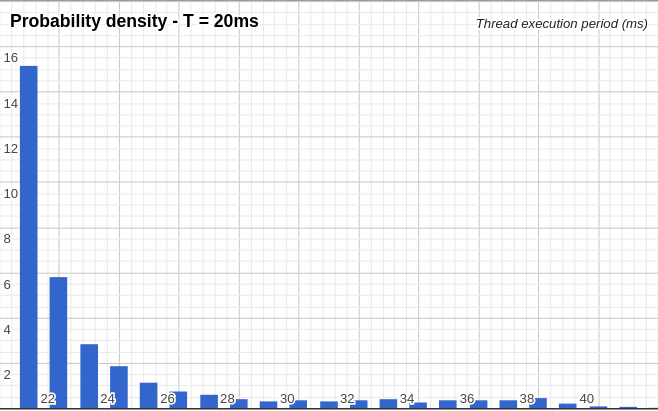
\includegraphics[width=\textwidth]{Pictures/dsp20.png}}
    \label{fig:dsp20}
    \rule{16em}{0.5pt}
    \caption[Waveform on power-linel]{Waveform on power-line}
  \end{minipage}
  \hfill%
  \begin{minipage}[c]{.46\linewidth}
  \centering
    \scalebox{1}{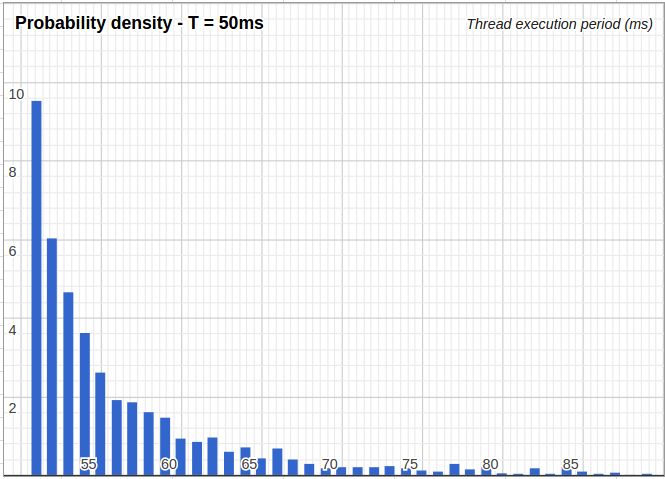
\includegraphics[width=\textwidth]{Pictures/dsp50.png}}
    \label{fig:dsp50}
    \rule{16em}{0.5pt}
    \caption[Waveform on power-linel]{Waveform on power-line}
  \end{minipage}
\end{figure}

\item Android threads can't reach lower period than 8ms but with an elevate variance, as we can see in .

\item Performing statistical analysis, for each execution period and plotting the effective period distribution and variance, we can consider 30ms as safe.

\item Even if the I2C bus speed clock should be 400kHz - according to the Ara MDK documentation - the effective clock rate is 133kHz.
On other hand, even if the kernel driver limits I/O operations to 512 bytes, the bus gets corrupted trying to transfer more than 350 bytes per operation.
\end{itemize}

\subsubsection{Conclusion}  \label{conclusion-ara}
According to , we should design our VLC receiver module to taking account an effective bit-rate of 92,4 kbps and will developed the Android application with a module polling thread period to 30ms and an I2C transaction . 


\subsection{Ara benchmark}

In addition to \ref{result-ara}, we should be sure that a normal to extensive modular smartphone won't affect VLC module performances, even if the app run in background mode. In this case, the Android CPU governor will reduce the priority of our app, giving it less resources or stopping it if necessary.

In order to do that, we use a benchmark application that would simulate typical smartphone use-case : web browsing, shot-message writing, video playing or games.

During the stress tests, both CPU load and repartitions over running process, and RAM usage are monitored.

\begin{figure}[h]
  \begin{minipage}[c]{.46\linewidth}
    \centering
    \scalebox{0.9}{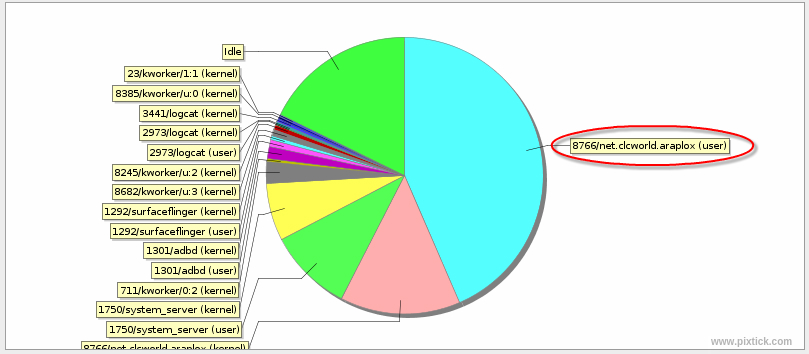
\includegraphics[width=\textwidth]{Pictures/cpu-singleapp.jpg}}
    \label{fig:cpu-single}
    \rule{16em}{0.5pt}
    \caption[Waveform on power-linel]{Waveform on power-line}
  \end{minipage}
  \hfill%
  \begin{minipage}[c]{.46\linewidth}
  \centering
    \scalebox{0.9}{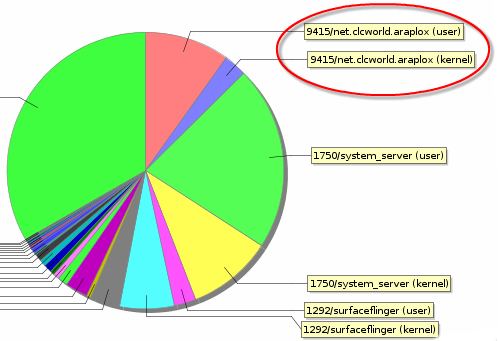
\includegraphics[width=\textwidth]{Pictures/cpu-loadapp.jpg}}
    \label{fig:cpu-load}
    \rule{16em}{0.5pt}
    \caption[Waveform on power-linel]{Waveform on power-line}
  \end{minipage}
\end{figure}

For each case, except the video game that made freeze and crash the Ara platform, results where exactly the same than with a single activity - ie. just our application - and we achieve the same bit-rate.

\subsubsection{Conclusion}


%----------------------------------------------------------------------------------------
%	Receiver circuit design
%----------------------------------------------------------------------------------------

\section{Receiver circuit design}

\subsection{Needs description}
\subsection{Photodiode}
\subsection{1st AOP : Current to tension converter}
\subsection{2sd: Low Pass filter}
\subsection{Gain}

%----------------------------------------------------------------------------------------
%	Emitter driver
%----------------------------------------------------------------------------------------

\section{Emitter driver}

\subsection{OOK modulation}
\subsection{4B6B Line coding}
\subsection{Algorithm}


%----------------------------------------------------------------------------------------
%	Receiver CAN and Buffer
%----------------------------------------------------------------------------------------

\section{Receiver CAN and Buffer}

\subsection{Digitalization}
\subsection{Decoding}
\subsection{Buffering}
\subsection{Input/output}

%----------------------------------------------------------------------------------------
%	Ara Android App
%----------------------------------------------------------------------------------------

\section{Ara Android App}

In this part, we describe the Android application that we have developed, to support our VLC receiver module.

\subsection{Application structure and operations}
Our application as been developed used Google Android API 18, to be compliant with the operating system version which has been installed on the AP Board.

The application package has been called respecting Java name convention : edu.upc.entel.wng.vlcAraModule and content 3 classes :

\begin{itemize}
\item VLCAraActivity : initialize the application and user interface. It surcharges the Activity class , as requested by the Android API.
\item Sensor : define and perform operations to communicate with our module such as I2C bus initialization, data polling as well as handling and message with the User Interface (UI).
\item VlcLogger : this class realize logging operation saving received data on the board internal storage or an external SD Card.
\end{itemize}

Application workflow is quiet simple :
\begin{enumerate}
\item Initialize and start the application main Activity.
\item Setup the I2C Bus.
\item Initialize the logger and create a log file.
\item Start the \textbf{Sensor} thread that poll I2C bus at defined interval and send the result to the android activity. 
\item Handle Sensor thread messaging and user interaction.
\end{enumerate}

\subsection{User Interface}

The application user interface as few components as defined in the XML activity layout description file :
\begin{itemize}
\item EditText field: used to display received bits.
\item "Clear" and "Save" Button :
\end{itemize}

Each component are placed in a horizontal layout container.

\subsection{I2C JNI interface}

As the Android Java API for the Ara Module Development Kit is the same as the standard API, we need to implement additional components in order to access the low level hardware such as the GPIO or the I2C bus.
The Ara MDK is provided with an operating system level driver, developed in C, that can be used to configure, read and write date, in a simple way.
However, this C interface, can't be directly used through the Java API. In order to give the possibility to perform I2C operations in our Android application, we develop a JNI interface that would wrap the C driver into a Java package.
So we define 2 Java classes : 
\begin{itemize}
\item I2CManager : it configures the i2c bus, by using UNIX I2C kernel driver and execute I2CTransaction.
\item I2CTransaction : it represents read or write operation on the bus.
\end{itemize}

Class methods are detailed in the Anexxe.

\subsection{Results}
\subsection{Interpretation} 
% Results

\chapter{Results} % Main chapter title

\label{Results} % For referencing the chapter elsewhere, use \ref{Chapter1} 

\lhead{Chapter 6. \emph{Tests and results}} % This is for the header on each page - perhaps a shortened title

In this chapter, we will describe and discuss our experimental results in order to validate our system and bring it to face to previous studies.
 
%----------------------------------------------------------------------------------------
%	METHODOLOGY
%----------------------------------------------------------------------------------------

\section{Experimental setup}

We propose to evaluate different aspects and characteristics of our system considering an indoor communication situation avoiding sunlight perturbations.

In addition, we consider different cases: with or without ambient light interferences, Manchester or 4B6B coding, changing the clock rate and the emitter distance from the receiver. 

\section{Validation method}

The receiver was placed in a fix position, while the LED light source keep mobile. In that way, the distance between the emitter and the receiver can  be changed. To keep the measure consistent, we place a luxmeter, just near the receiver to approximate the effective illumination.

During the probes, both emitter and receiver micro-controller were connected with their debugging interface to a laptop, on a side to change the LED driver parameters, and on other side to visualize and record received data at different place of our system. 

In addition, we used on oscilloscope to check the circuit output and control the signal generated by the emitter micro-controller.

The emitter light was alimented with a 28 Volts power supply and the LED Driver has been programmed to send periodically a 16-bits counter value, with the pattern defined in \ref{frame}.

About the distance/illumination, probes have been realized in a range of 75 to 300 centimeters to match an indoor possible usage. On other side, the clock frequency has been limited to 560kHz, considering the ADC sampling rate - 1,1 MSPS - and the Nyquist-Shannon sampling theorem : 
\begin{equation}
f_{Nyquist}  = \frac{f_{sampling}}{2}
\label{eq:nyquist}
\end{equation}

\begin{figure}[htbp]
  \centering
    \makebox[\textwidth][c]{
      \scalebox{0.4}{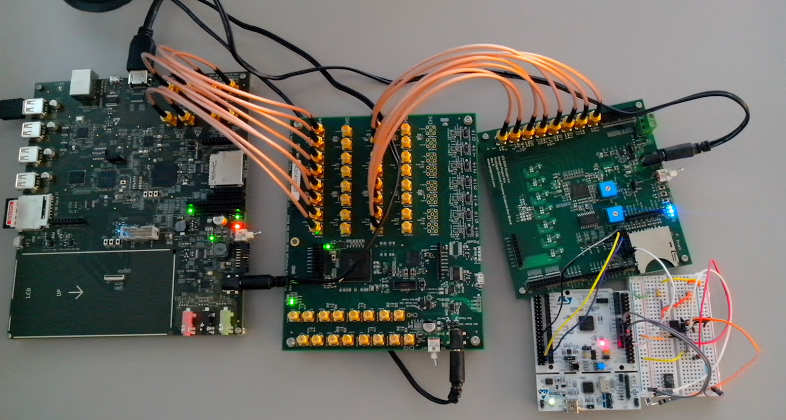
\includegraphics{Pictures/receiver_setup.jpg}
    }}
    \rule{35em}{0.5pt}
  \caption[The Ara MDK and its VLC receiver module]{The Ara MDK and its VLC receiver module}
  \label{fig:receiver}
\end{figure}

\begin{figure}[htbp]
	\centering
	\makebox[\textwidth][c]{
		\scalebox{0.3}{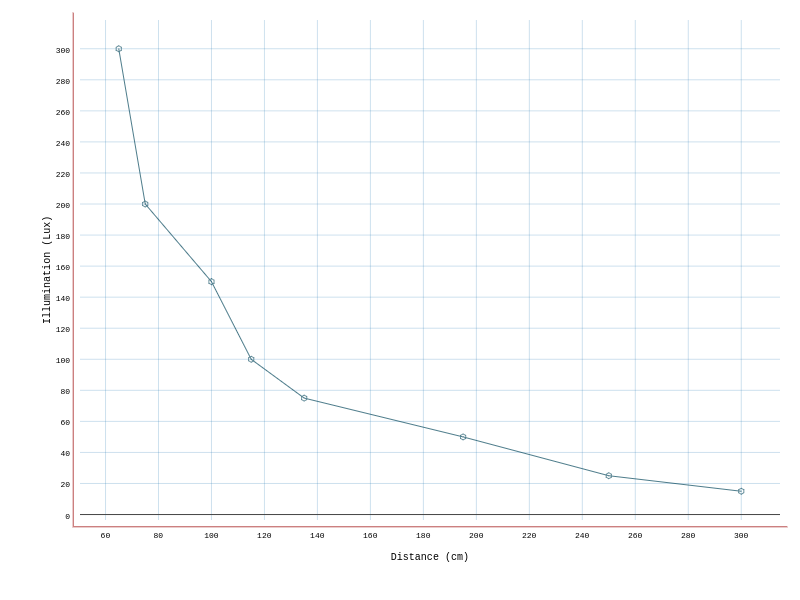
\includegraphics{Pictures/led.png}
	}}
		\rule{35em}{0.5pt}
		\caption{Receiver illumination over the distance}
		\label{fig:led}
	\end{figure}

\section{Circuit Evaluation}

The received signal was measured at different steps of the analogical processing, using the 2 oscilloscope channels at different points of our circuit. The high-pass filter and adjustments made on the receiver front-end circuit are satisfactory, and improve the signal quality before sampling.

\begin{figure}[htbp]
	\centering
	\makebox[\textwidth][c]{
		\scalebox{0.6}{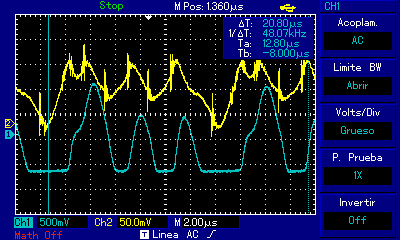
\includegraphics{Pictures/circuit-compare.png}
	}}
		\rule{35em}{0.5pt}
		\caption[In yellow the signal just after the TIA. In blue, the signal after analogical filtering - 2,5 meter distance]{In yellow the signal just after the TIA. In blue, the signal after analogical filtering - 2,5 meter distance}
		\label{fig:circuit-compare}
	\end{figure}
	
\section{Digitalization and demodulation}

In order evaluate our demodulation and digital processing algorithms, we plot the sampled signal and the bits obtained after computation. We can see in the figure \ref{fig:numeric} that it is correct and we can get rid of signal attenuation due to circuit latency.
\begin{figure}[htbp]
	\centering
	\makebox[\textwidth][c]{
		\scalebox{0.4}{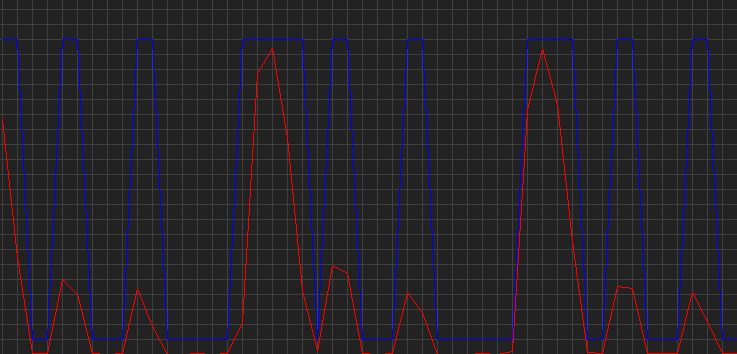
\includegraphics{Pictures/numerized.png}
	}}
		\rule{35em}{0.5pt}
		\caption{In red the signal sampled. In blue, the bits computed after digital processing and demodulation}
		\label{fig:numeric}
	\end{figure}

\section{Bit Error Rate}

In digital transmission, the number of bit errors is the number of received bits of a data stream over a communication channel that have been altered due to noise, interference, distortion or bit synchronization errors.

As we know exactly the emitted bit-sequence and the decoded sequence, we were able to compute it, for different illumination level and clock-rate, using Manchester or 4B6B coding.

\subsection{4B6B}

\begin{table}[htbp]
\begin{center}
\begin{tabular}{|c|c|c|}
  \hline
  clock rate (kHz) & bitrate (kbps) & BER \\
  \hline
  100 & 67 & $<$ 10$^-4$ \\
  160 & 107 & $<$ 10$^-4$ \\
  240 & 160 & 3.10$^-4$ \\
  380 & 253 & 6.10$^-4$ \\
  560 & 373 & 2.10$^-2$ \\
  \hline
\end{tabular}
\end{center}
\caption{Bit Error Rate for different clock rate at 2,5 meters, using 4B6B coding}
\label{tab:ber}
\end{table}

Considering table \ref{tab:ber} 2,5 meters distance and 10$^-3$ as admissible BER, we can assume that using a 380kHz clock rate can be used for a correct transmission using 4B6B.

In that case, with 4B6B coding, we obtain a raw throughput of 253 kbps.

\subsection{Manchester}
Using Manchester coding, we obtained a surge of the bit error rate when the illumination is lower than 100 Lux. Analyzing the signal at the ADC input, we put in evidence that this is due to wave attenuation : isolated bit, just after long sequences are not detected, as visible in the figure \ref{fig:manchester-problem}.

\begin{table}[htbp]
\begin{center}
\begin{tabular}{|c|c|c|}
  \hline
  clock rate (kHz) & bitrate (kbps) & BER \\
  \hline
  100 & 50 & $<$ 10$^-4$ \\
  160 & 80 & $<$ 10$^-4$ \\
  240 & 120 & 8.10$^-4$ \\
  380 & 190 & 4.10$^-2$ \\
  560 & 280 & $>$ 10$^-1$ \\
  \hline
\end{tabular}
\end{center}
\caption{Bit Error Rate for different clock rate at 2,5 meters, using Manchester coding}
\label{tab:ber-manchester}
\end{table}

\begin{figure}[htbp]
	\centering
	\makebox[\textwidth][c]{
		\scalebox{0.6}{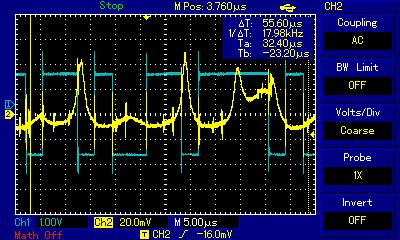
\includegraphics{Pictures/manchester-prob.jpg}
	}}
		\rule{35em}{0.5pt}
		\caption
        {In blue, the signal generated by the LED driver. In yellow, the signal after our circuit - 2,5 meter distance - 360kHz}
		\label{fig:manchester-problem}
	\end{figure}
    
 
%----------------------------------------------------------------------------------------
%	RESULTS AND INTERPRETATION-----------------------

%-----------------------------------------------------------------
\section{Discussion}

Regarding previous results, we were able to validate our proposal. We can achieve a reliable transmission between a commercial LED and the modular smartphone at a suitable distance for indoor usage.

Comparing our  module for Ara platform with previous system, such \citep{phycomp}, or other proposal using the smartphone camera and rolling shutter effect  \citep{rolling}, we obtained and recorded an higher bitrate, up to 253 kbps.
\citep{phycomp}
% Conclusion

\chapter{Conclusion}

\label{Conclusion}

\lhead{Chapter 7. \emph{Conclusion}}

%----------------------------------------------------------------------------------------
%	Achieved work
%----------------------------------------------------------------------------------------

\section{Achieved work}

%----------------------------------------------------------------------------------------
%	Future works
%----------------------------------------------------------------------------------------

\section{Future works} 

%----------------------------------------------------------------------------------------
%	THESIS CONTENT - APPENDICES
%----------------------------------------------------------------------------------------

\addtocontents{toc}{\vspace{2em}} % Add a gap in the Contents, for aesthetics


%----------------------------------------------------------------------------------------
%	BIBLIOGRAPHY
%----------------------------------------------------------------------------------------

\label{Bibliography}

\lhead{\emph{Bibliography}} % Change the page header to say "Bibliography"

\bibliographystyle{unsrtnat} % Use the "unsrtnat" BibTeX style for formatting the Bibliography

\bibliography{Bibliography} % The references (bibliography) information are stored in the file named "Bibliography.bib"

\appendix % Cue to tell LaTeX that the following 'chapters' are Appendices

% Ara development kit documentation

\chapter{Ara development kit documentation}

\label{Ara}

\lhead{Appendix A. \emph{Ara development kit documentation}}
%\includepdf[pages=-, scale=.85]{Appendices/Ara.pdf}
\includepdf[pages=1,pagecommand={},offset=2.5cm -3cm]{Appendices/Ara.pdf}
\includepdf[pages=2,pagecommand={},offset=2.5cm -3cm]{Appendices/Ara.pdf}
\includepdf[pages=3,pagecommand={},offset=2.5cm -3cm]{Appendices/Ara.pdf}
\includepdf[pages=4,pagecommand={},offset=2.5cm -3cm]{Appendices/Ara.pdf}
\clearpage
% Circuit Schematics

\chapter{Circuit Schematics}

\label{Circuit}

\lhead{Appendix B. \emph{Circuit Schematics}}

\begin{figure}[htbp]
  \centering
  \makebox[\textwidth][c]{
    \scalebox{0.55}{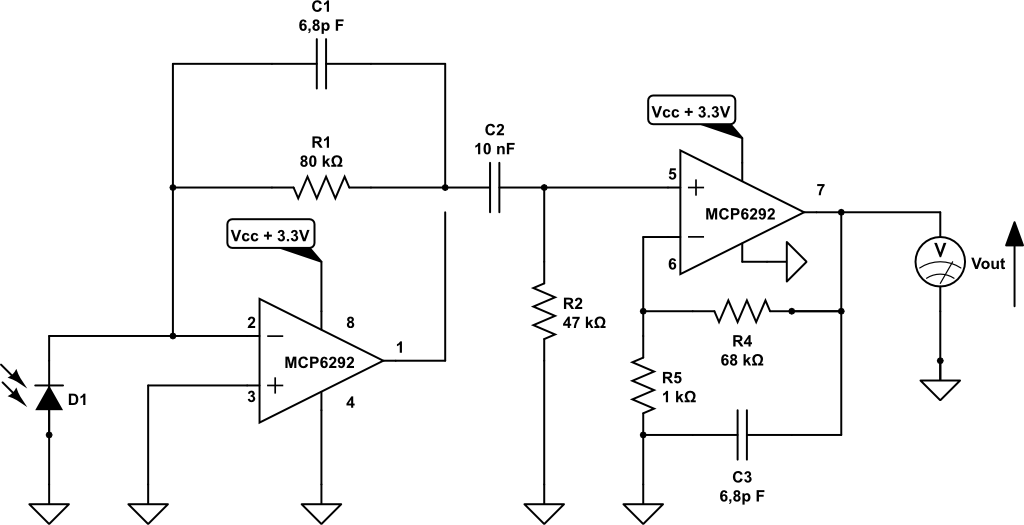
\includegraphics{Pictures/vlc-receiver-circuit-v3.png}}
   }
  \rule{35em}{0.5pt}
  \caption[VLC Receiver front-end circuit]{VLC Receiver front-end circuit}
  \label{fig:RxCircuit}
\end{figure}

% Emitter software sources

\chapter{Emitter software sources}

\label{Emitter}

\lhead{Appendix C. \emph{Emitter software sources}}

    \lstinputlisting[language=C, caption=main.c, escapeinside={\%*}{*)}{\#*}, label=main.c]{CodeEmitter/main.c}

    \lstinputlisting[language=C, caption=i2c.c ,label=i2c.c, escapeinside={\%*}{*)}{\#*}]{CodeEmitter/4b6b.c}

    \lstinputlisting[language=C, caption=fifo.c ,label=fifo.c, escapeinside={\%*}{*)}{\#*}]{CodeEmitter/4b6b.h}


% Receiver software sources

\chapter{Receiver software sources}

\label{codereceiver}

\lhead{Appendix D. \emph{Receiver software sources}}


    \lstinputlisting[language=C, caption=main.c, escapeinside={\%*}{*)}{\#*}, label=rmain.c]{CodeReceiver/main.c}

  
    \lstinputlisting[language=C, caption=i2c.c ,label=ri2c.c, escapeinside={\%*}{*)}{\#*}]{CodeReceiver/i2c.c}

    \lstinputlisting[language=C, caption=fifo.c ,label=rfifo.c, escapeinside={\%*}{*)}{\#*}]{CodeReceiver/fifo.c}

    \lstinputlisting[language=C, caption=dma.c ,label=rdma.c, escapeinside={\%*}{*)}{\#*}]{CodeReceiver/dma.c}

    \lstinputlisting[language=C, caption=adc.c ,label=radc.c, escapeinside={\%*}{*)}{\#*}]{CodeReceiver/adc.c}

% Java software sources

\chapter{Java software sources}

\label{Java}

\lhead{Appendix G. \emph{Android VLC application sources}}

\lstinputlisting[language=C, caption=Sensor.java, escapeinside={\%*}{*)}{\#*}, label=Sensor.java]{CodeAndroid/Sensor.java}

\lstinputlisting[language=C, caption=VlcLogger.java ,label=IVlcLogger.java, escapeinside={\%*}{*)}{\#*}]{CodeAndroid/VlcLogger.java}

\lstinputlisting[language=C, caption=VlcAraActivity.java ,label=VlcAraActivity.java, escapeinside={\%*}{*)}{\#*}]{CodeAndroid/VlcAraActivity.java}

\lstinputlisting[language=XML, caption=AndroidManifest.xml ,label=AndroidManifest.xml, escapeinside={\%*}{*)}{\#*}]{CodeAndroid/AndroidManifest.xml}
% JNI software sources

\chapter{JNI software sources}

\label{JNI}

\lhead{Appendix F. \emph{JNI software sources}}

\lstinputlisting[language=C, caption=jni-i2c.c, escapeinside={\%*}{*)}{\#*}, label=jni.c]{CodeJNI/jni.cpp}

\lstinputlisting[language=C, caption=I2cManager.java ,label=I2cManager.java, escapeinside={\%*}{*)}{\#*}]{CodeJNI/I2cManager.java}

\lstinputlisting[language=C, caption=I2cTransaction.java ,label=I2cTransaction.java, escapeinside={\%*}{*)}{\#*}]{CodeJNI/I2cTransaction.java}

\lstinputlisting[language=C, caption=I2cService.java ,label=I2cService.java, escapeinside={\%*}{*)}{\#*}]{CodeJNI/I2cService.java}
% Circuit Schematics

\chapter{STM32L0 Nucleo Schmeatic}

\label{stm32}

\lhead{Appendix E. \emph{STM32L0 Nucleo Schmeatic}}

\begin{figure}[htbp]
  \centering
  \makebox[\textwidth][c]{
    \scalebox{0.6}{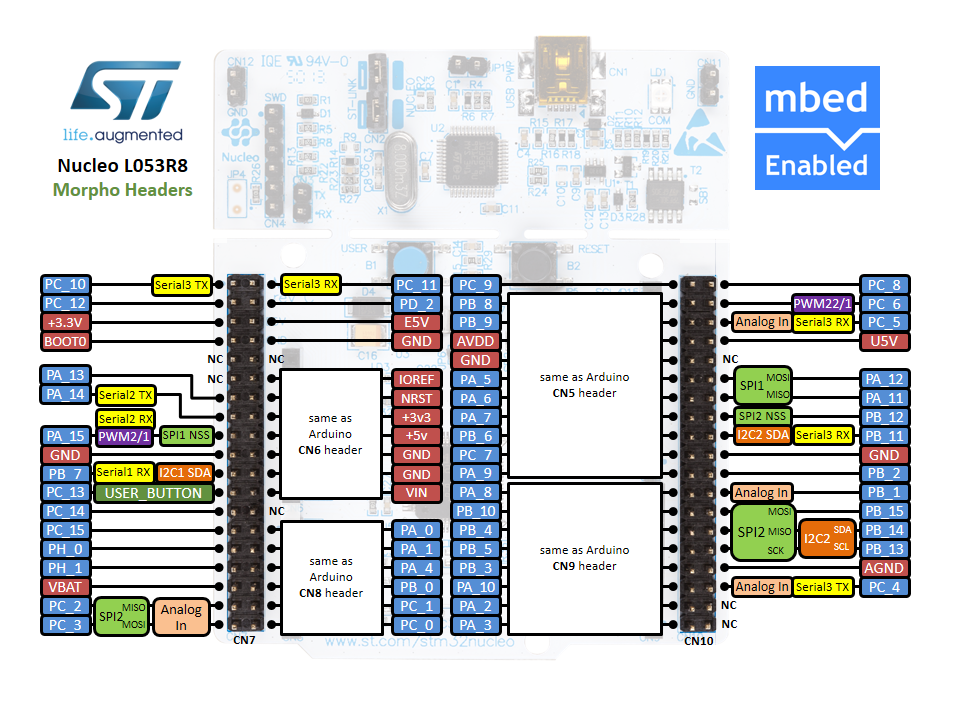
\includegraphics{Pictures/mcupin.png}}
   }
  \rule{35em}{0.5pt}
  \caption[STM32L0 Nucleo Schmeatic]{STM32L0 Nucleo Schematic}
  \label{fig:RxCircuit}
\end{figure}


\addtocontents{toc}{\vspace{2em}} % Add a gap in the Contents, for aesthetics

\backmatter

\end{document}